Một miền cần chia đủ nhỏ để phù hợp với một nhóm cụ thể. Để đạt được điều này, chúng ta cần xác định rõ ranh giới giữa các ngữ cảnh. \emph{Bối cảnh bị giới hạn (Bounded Context)} giúp xác định rõ các ranh giới, chia miền thành các phần độc lập để giải quyết sự phức tạp trong mô hình doanh nghiệp. Bối cảnh bị giới hạn tạo ra các mô hình khác nhau cho các lĩnh vực khác nhau của miền. Bối cảnh bị giới hạn thể hiện phạm vi kinh doanh của dịch vụ.

\begin{figure}[H]

    \centering

    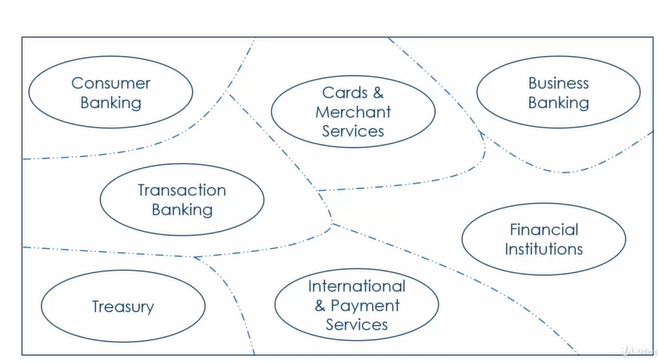
\includegraphics[scale = 1]{pictures/boi_canh_gioi_han/main.png}

    \caption{Ví dụ về bối cảnh bị giới hạn trong một ngân hàng}

\end{figure}

\subsubsection{Cách xác định bối cảnh bị giới hạn}

Để có thể xác định được bối cảnh bị giới hạn chúng ta có thể xem xét:

\begin{itemize}

    \item Dựa vào việc phân chia các miền phụ.

    \item Dựa vào sơ đồ cấu trúc tổ chức các phòng ban của doanh nghiệp.

    \item Dựa vào modules của các ứng dụng kiến trúc nguyên khối (nếu việc phân chia tốt).

    \item Dựa vào trách nhiệm và hoạt động của chuyên gia miền .

\end{itemize}

% \subsubsection{Áp dụng xác định bối cảnh bị giới hạn trong đồ án này}

% \subsubsection{Áp dụng xác định bối cảnh bị giới hạn trong đồ án này}

% \subsubsection{Áp dụng xác định bối cảnh bị giới hạn trong đồ án này}

% \subsubsection{Áp dụng xác định bối cảnh bị giới hạn trong đồ án này}

% \subsubsection{Áp dụng xác định bối cảnh bị giới hạn trong đồ án này}

% \subsubsection{Áp dụng xác định bối cảnh bị giới hạn trong đồ án này}

% \subsubsection{Áp dụng xác định bối cảnh bị giới hạn trong đồ án này}

% \subsubsection{Áp dụng xác định bối cảnh bị giới hạn trong đồ án này}

% \subsubsection{Áp dụng xác định bối cảnh bị giới hạn trong đồ án này}

% \subsubsection{Áp dụng xác định bối cảnh bị giới hạn trong đồ án này}

% \subsubsection{Áp dụng xác định bối cảnh bị giới hạn trong đồ án này}

% \subsubsection{Áp dụng xác định bối cảnh bị giới hạn trong đồ án này}

%!<! - - Hướng dẫn 5/10 - - >

%!<! - - Hướng dẫn 5/10 - - >

%!<! - - Hướng dẫn 5/10 - - >

%!<! - - Hướng dẫn 5/10 - - >

%!<! - - Hướng dẫn 5/10 - - >

%!<! - - Hướng dẫn 5/10 - - >

%!<! - - Hướng dẫn 5/10 - - >

%!<! - - Hướng dẫn 5/10 - - >

%!<! - - Hướng dẫn 5/10 - - >
